\documentclass[11pt]{beamer}
\usetheme{Luebeck}
\usepackage[utf8]{inputenc}
\usepackage[english]{babel}
\usepackage{amsmath}
\usepackage{amsfonts}
\usepackage{amssymb}
\usepackage{caption}

\usepackage{subfig}
\captionsetup{labelformat=empty}
\usepackage{xcolor}

\usepackage[style=alphabetic,backend=biber]{biblatex}
\addbibresource{slides.bib}

%% Defining new colors %%
\definecolor{Orange}{RGB}{255,140,30}
\setbeamercolor{normal text}{fg=black,bg=white}
\setbeamercolor{structure}{fg=Orange}
\setbeamercolor{palette quaternary}{fg=white, bg=black}

%% REVISION MACROS

\newcommand{\todo}[1]{\textcolor{red}{\textbf{ToDo}\ifx&#1&\else ~[\emph{#1} ]~\fi}}
\newcommand{\fixme}[1]{\textcolor{purple}{\textbf{FixMe}\ifx&#1&\else ~[ \emph{#1} ]~\fi}}


%% Tikz for picture drawing %%
\usepackage{tikz}
\usetikzlibrary{arrows}

%%
\title{Data Skew in Map-Reduce}
\subtitle{Cloud and Big Data - M1RI}
\date{April 4th, 2017}
\author{Florestan De Moor, Jérémy Thibault}

\titlegraphic{
\includegraphics[scale=0.6]{ens} \hspace{2cm} 
\includegraphics[scale=0.15]{univ-rennes1}}

%%
\useoutertheme[subsection=false]{smoothbars}

\setbeamertemplate{footline}{\hspace*{\fill}\insertframenumber/\inserttotalframenumber\hspace*{0.3cm}}
\setbeamerfont{footline}{series=\bfseries,size=\fontsize{8}{12}\selectfont}

\setbeamertemplate{navigation symbols}{}

\setbeamertemplate{caption}{\raggedright\insertcaption\par}

\setbeamertemplate{bibliography item}[text]

\graphicspath{{img/}}

\begin{document}

%%%%%%%%%%%%%%%%%%%%%%%%%%%%%%%%%%%%%%%%%%%%%%%%%%%%%%%%%%%%

\begin{frame}
    \maketitle
\end{frame}

%%%%%%%%%%%%%%%%%%%%%%%%%%%%%%%%%%%%%%%%%%%%%%%%%%%%%%%%%%%%

\section{Introduction}

%%%%%%%%%%%%%%%%%%%%%%%%%%%%%%%%%%%%%%%%

\begin{frame}{Outline}
    \tableofcontents
\end{frame}

%%%%%%%%%%%%%%%%%%%%%%%%%%%%%%%%%%%%%%%%%%%%%%%%%%%%%%%%%%%%

\section{Data Skew Challenges}

%%%%%%%%%%%%%%%%%%%%%%%%%%%%%%%%%%%%%%%%

\subsection{Definition and Challenges}

%%%%%%%%%%%%%%%%%%%%

\begin{frame}{Skewness Definition \footnote{\url{https://en.wikipedia.org/wiki/Skewness}}}

\textbf{Asymmetry} of a probability distribution or a dataset distribution

\vfill

\begin{exampleblock}{}
\begin{figure}
    \centering
    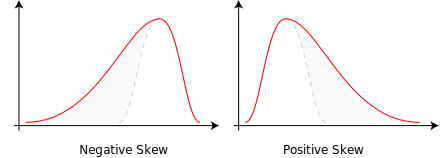
\includegraphics[width=0.7\textwidth]{skewness}
    \caption{Example of negative and positive skewness in a probability distribution}
    \label{img:skewness_def}
\end{figure}
\end{exampleblock}

\end{frame}

%%%%%%%%%%%%%%%%%%%%

\begin{frame}{Challenges \cite{Kwon11astudy} }

\begin{alertblock}{Data skew consequences}

$\bullet$ Highly variable task runtimes

$\bullet$ Computational load unbalance among map / reduce tasks

$\quad \longrightarrow$ \emph{Map-skew} and \emph{Reduce-skew}

$\bullet$ A few tasks cause the job to take much longer
\end{alertblock}

\vfill

\begin{block}{What about speculative execution?}

Efficient to mitigate performance skew of physical nodes

But here: speculative tasks runtime $\simeq$ original tasks runtime

$\longrightarrow$ Not a solution for data skew

\end{block}

\end{frame}

%%%%%%%%%%%%%%%%%%%%

\subsection{Map-Skew Examples}

\begin{frame}{Map-Skew Examples \cite{Kwon11astudy}}

$\bullet$ \textbf{Expensive Record}

few words

\vfill

$\bullet$ \textbf{Heterogeneous Maps}

few words

\vfill

$\bullet$ \textbf{Non-Homomorphic Map}

few words

\end{frame}

%%%%%%%%%%%%%%%%%%%%%%%%%%%%%%%%%%%%%%%%

\subsection{Reduce-Skew Examples}

%%%%%%%%%%%%%%%%%%%%

\begin{frame}{Reduce-Skew Examples \cite{Kwon11astudy}}

$\bullet$ \textbf{Partitioning Skew}

few words

\vfill

$\bullet$ \textbf{Expensive Input}

few words

\end{frame}

%%%%%%%%%%%%%%%%%%%%%%%%%%%%%%%%%%%%%%%%%%%%%%%%%%%%%%%%%%%%

\section{How to handle data skew in Map-Reduce?}

%%%%%%%%%%%%%%%%%%%%%%%%%%%%%%%%%%%%%%%%%%%%%%%%%%%%%%%%%%%%

\subsection{Overview of some existing algorithms}

%%%%%%%%%%%%%%%%%%%%%%%%%%%%%%%%%%%%%%%%

\subsection{Focus on an algorithm (Skewtune?)}

%%%%%%%%%%%%%%%%%%%%

\begin{frame}
\end{frame}

%%%%%%%%%%%%%%%%%%%%%%%%%%%%%%%%%%%%%%%%%%%%%%%%%%%%%%%%%%%%

\section{Conclusion}

%%%%%%%%%%%%%%%%%%%%

\begin{frame}
    \cite{Kwon11astudy}
    \cite{Kwon:2012:SMS:2213836.2213840}
    \cite{gufler2011handling}
    \cite{ibrahim:hal-00822973}
\end{frame}

%%%%%%%%%%%%%%%%%%%%

\begin{frame}[allowframebreaks]{References}
    \printbibliography
\end{frame}

%%%%%%%%%%%%%%%%%%%%%%%%%%%%%%%%%%%%%%%%%%%%%%%%%%%%%%%%%%%%

\end{document}
